%! Author = chrystal
%! Date = 06.12.19

% Preamble
\documentclass[11pt]{article}

% Packages
\usepackage{amsmath}
\usepackage{graphicx}

\chapter{Factor Analysis}

\begin{section}{Variance and Covariance}

    \subsection{Varaince-Covariance-matrix}

    \paragraph{Factor Analysis} Reduces the original number of attributes to a smaller number of factors, 
    each containing a set of attributes that hang together

    \paragraph{Covariance} Hints if the result of one variable gives you information about the other $\rightarrow$
    A small standard deviation will cause a covariance near zero.
    $cov(x,y) = \frac{1}{n-1} \sum_{i=1}^n (x_i - mean_x) \times (y_i - mean_y)$ \\
    $cov(x,x) = var(x)$

    \paragraph{Variance-Covariance-matrix} square matrix that contains the variances and covariances associated with several variables x and y.
    Scatter-Plotting the Variance-Covariance-Matrix every dot represents one person, with one axes representing one variable.

    $$ S =
    \begin{bmatrix}
        $cov(x,x)$
        & $cov(x,y)$ \\
        a $cov(y,x)$
        & $cov(y,y)$
    \end{bmatrix}
    $$
    
    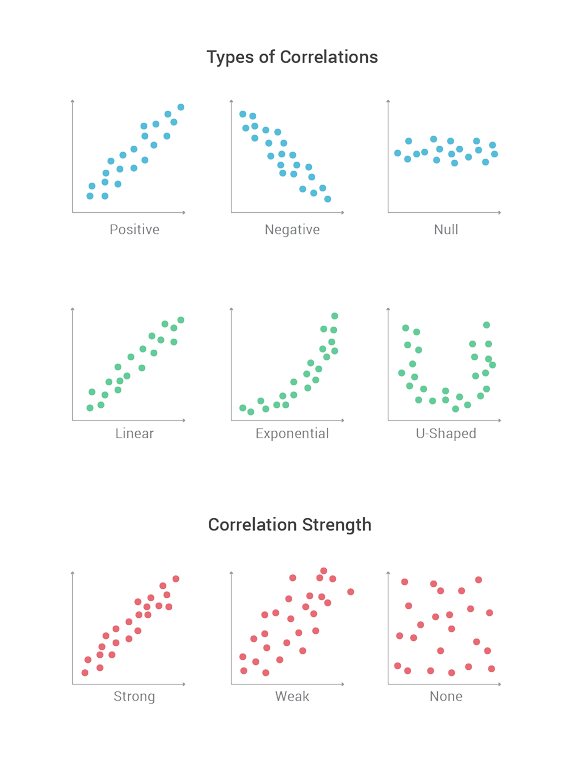
\includegraphics{../assets/scatterplots.png}

    \paragraph{Example} \textit{
    x, y: liking of course x, y. X having a high variance, Y a very low. Therefore both Covariances will be very low as well.
    A data set with low variance will not explain much $\rightarrow$ Correlation of null
    
    $$ S =
    \begin{bmatrix}
        16
        & 2.5 \\
        a 2.5
        & 2
    \end{bmatrix}
    $$
    }
    
    \paragraph{Principal component} The principal components analysis allows to compute factor weights in order to extract the maximum possible variance
    from the original variables and to continue factoring until there is no more meaningful variance left
    $\rightarrow$ \textbf{Latent Variable} a variable, that can not be meassured directly.
    This analysis is widely used in the market segmentation: for example it allows to identify important consumers evaluations about different dimensions 
    of a product/service.
    From a statistical point of view, the aim of the factor analysis is to identify a reduced number of linear combinations of the original variables 
    that explain most of the variance of the same variables $X$, a weight $a$. Every linear combination is a function of all the original variables, 
    but it is correlated in particular to some of them
    $c=a_1 X_1+a_2 X_2+ ... +a_n X_n$

    The components or factors are not correlated among each other and their maximal number is equal to the number of original variables ($p$).
    The components explain a decreasing percentage of data variance. The higher the correlation of the original variables, the higher is the power of the factor analysis, 
    and the less information you loose by performing it
    
    \paragraph{Procedure} \textit{Identify gaps for new products} $\rightarrow$ Identify competitors $\rightarrow$ Identify important product dimensions for mapping
    $\rightarrow$ Use customer surveys to map competitors and yourself along these dimensions $\rightarrow$ Identifying Dimensions $\rightarrow$ Interpret Perceptual Map
    
    
\end{section}